%
% File acl-hlt2011.tex
%
% Contact: gdzhou@suda.edu.cn
%%
%% Based on the style files for ACL2008 by Joakim Nivre and Noah Smith
%% and that of ACL2010 by Jing-Shin Chang and Philipp Koehn


\documentclass[11pt]{article}
\usepackage{acl-hlt2011}
\usepackage{times}
\usepackage{latexsym}
\usepackage{amsmath}
\usepackage{multirow}
\usepackage{url}
\usepackage{graphicx}
\usepackage{synttree}
\bibliographystyle{acl}

\setlength\titlebox{6.5cm}    % Expanding the titlebox


\title{[x]}

\author{Someone \and Someone Else \and A Third \\
  Language Technologies Institute \\
  Carnegie Mellon University \\
  Pittsburgh, PA 15213\ \ USA \\
  {\tt \{x, y, z\}@cs.cmu.edu}}
\date{}


\begin{document}

\maketitle

\begin{abstract}
[x]
\end{abstract}


\section{Introduction}

[Some intro/drill-down paragraph(s): SCFG-based MT needs rules.  There are lots of ways to get rules.]

Some SCFG rule extraction techniques require only Viterbi word alignment links between the source and target sides of the input corpus \cite{Chiang-Hiero}, while methods based on linguistic constituency structure require the source and/or target side of the input to be parsed.  Among such techniques, most retain the dependency on Viterbi word alignments for each sentence \cite{GalleyEtAl-TransRule,ZollmannVenugopal-SyntaxAugmentedMT,Lavie-SSST,Chiang-SourceAndTarget} while others make use of a general, corpus-level statistical lexicon instead of individual alignment links \cite{ZhechevWay-DCUNodeAlignment}.  [There are also constraints on the form, size, etc. of the rules you get in each.]

This paper describes a new, general-purpose rule extractor intended for cases in which two parse trees and Viterbi word alignment links are provided for each sentence, although compatibility with single-parse-tree extraction methods can be achieved by supplying a flat ``dummy'' parse for the missing tree.  Our framework for rule extraction is thus most similar to the Stat-XFER system \cite{Lavie-SSST,AmbatiEtAl-ts2ts} and the tree-to-tree situation considered by \newcite{Chiang-SourceAndTarget}.  However, we significantly broaden the scope of allowable rules compared to the Stat-XFER heuristics, and our approach differs from Chiang's system in its respect of the linguistic constituency constraints expressed in the input tree structure.  In summary, we attempt to extract the greatest number of syntactically motivated rules as possible while not allowing them to violate explicit constituent boundaries on either the source or target side.  This is achieved by allowing the introduction of virtual nodes, by allowing multiple decompositions of the same tree pair, and by allowing extraction of SCFG rules beyond the minimial set required to re-generate the tree pair.

[A bit about where we're going in the rest of the paper?]


\section{Rule Extraction Algorithm}

We begin with a parallel sentence consisting of a source-side parse tree $S$, a target-side parse tree $T$, and a Viterbi word alignment between the trees' leaves.  A sample sentence of this type is shown in Figure \ref{Fig-AlignedTreePair}.  Our goal is to extract a number of SCFG rules that are licensed by this input.

\begin{figure*}[tbh!]
\begin{center}
\scalebox{0.8}{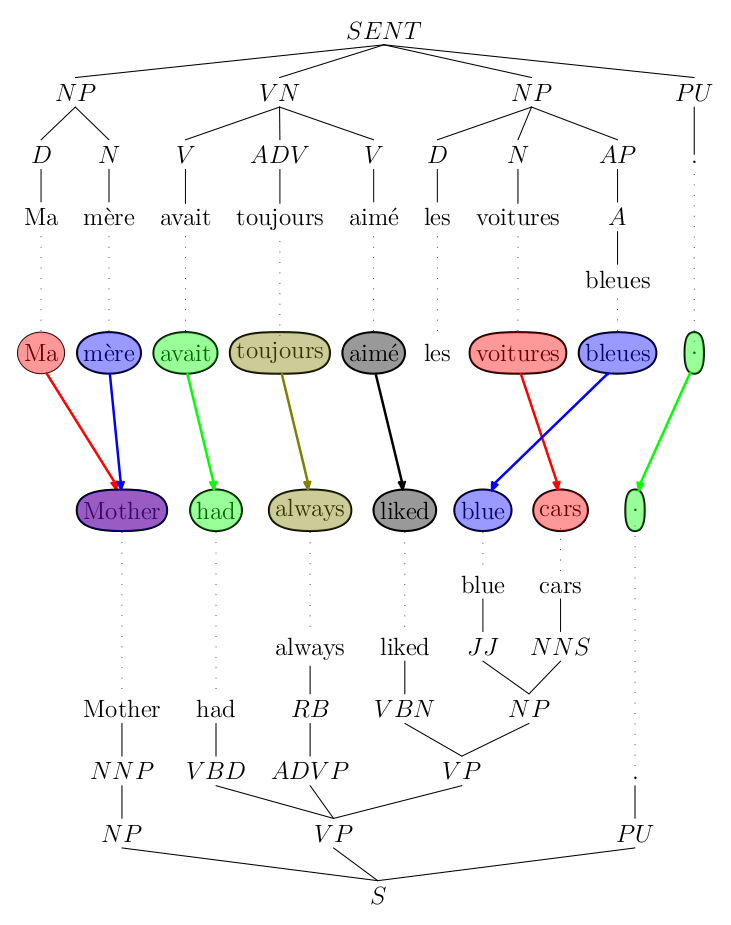
\includegraphics{rule-extr-1}}
\end{center}
\caption{\label{Fig-AlignedTreePair} Sample input for our rule extraction algorithm.  It consists of a source-side parse tree (French) and a target-side parse tree (English) connected by a Viterbi word alignment.}
\end{figure*}

\subsection{Node Alignment}

Our algorithm first computes a node alignment between the parallel trees.  A node $s$ in tree $S$ is aligned to a node $t$ in tree $T$ if the following constraints are met.  First, all words in the yield of $s$ must either be aligned to words within the yield of $t$, or they must be unaligned.  Second, the reverse must also hold: all words in the yield of $t$ must be aligned to words within the yield of $s$ or again be unaligned.  This is analogous to the word-alignment consistency constraint of phrase-based SMT phrase extraction \cite{KoehnEtAl-PBSMT}.  As in phrase-based SMT, where a phrase in one language may be consistent with multiple possible phrases in the other language, we allow parse nodes in both trees to have multiple node alignments.  This is in contrast to one-derivation rule extractors such as that of \newcite{Lavie-SSST}, in which each node in $S$ may only be aligned to a single node in $T$ and vice versa.

In Figure \ref{Fig-AlignedTreePair}, for example, the NP dominating the French words {\it les voitures bleues} is aligned to the equivalent English NP node dominating {\it blue cars}.  As an example of multiple alignments, the French NP node {\it Ma m\`ere} aligns to both the NNP and NP nodes in English producing {\it Mother}.

Besides aligning existing nodes in both parse trees to the extent possible, we permit the introduction of ``virtual'' nodes into either tree as well.  Virtual nodes are created when two or more contiguous children of an existing node are aligned consistently to a node or a similar set of two or more contiguous children of a node in the opposite parse tree.  Virtual nodes may be aligned to ``original'' nodes in the opposite tree or to other virtual nodes.

In Figure \ref{Fig-AlignedTreePair}, the existing English NP node {\it blue cars} can be aligned to a new virtual node in French that dominates the N node {\it voitures} and the AP node {\it bleues}.  The virtual node is inserted as the parent of N and AP, and as the child of the NP node directly above.  In conjunction with node alignments between existing nodes, this means that the English NP {\it blue cars} is now aligned twice: once to the original French NP node and once to the virtual node N+AP.  We thus replicate the behavior of ``growing into the gaps'' from phrase-based SMT in the presence of unaligned words.  As another example, a virtual node in French covering the V node {\it avait} and the ADV node {\it toujours} could be created to align consistently with a virtual node in English covering the VBD node {\it had} and the ADVP node {\it always}.

Since virtual nodes are always created out of children of the same node, they always are consistent with the existing syntactic structure of the tree.  Within the constraints of the existing tree structure and word alignments, however, all possible virtual nodes could potentially be considered.  This is in keeping with our philosophy of allowing multiple alignments without violating constituent boundaries.  Near the top of the trees in Figure \ref{Fig-AlignedTreePair}, for example, French virtual nodes NP+VN+NP (aligned to English NP+VP) and VN+NP+PU (aligned to VP+PU) both exist, even though they overlap.  In our procedure, we do allow a limit to be placed the number of child nodes that can be combined into a virtual node.  Setting this limit to two, for instance, will constrain node alignment to the space of possible synchronous binarizations consistent with the Viterbi word alignments.

\subsection{Grammar Extraction}

Given the final set of node alignments between the source tree and the target tree, SCFG rules are obtained via a grammar extraction step.  Rule extraction proceeds in a depth-first manner, such that rules are extracted and cached for all descendents of a source node $s$ before rules in which $s$ is the left-hand side are considered. Extracting rules where source node $s$ is the left-hand side consists of two phases.  The first phase is decomposition of node $s$ into all distinct sets $D = \{d_1, d_2, \ldots, d_n\}$ of descendent nodes such that $D$ spans the entire yield of node $s$, such that $d_i \in D$ is node-aligned for all $i$, and such that $d_i$ has no ancestor $a$ where $a$ is a descendent of $s$ and $a$ is node-aligned.  Each $D$ thus represents the right-hand side of a minimal SCFG rule rooted at $s$.  The second phase involves composition of all rules derived from each element of $D$ subject to certain constraints.

Due to the introduction of overlapping virtual nodes, the decomposition step may involve finding multiple sets of decomposition points when there are multiple nodes with the same span at the same level of the tree.  To see how multiple such decompositions could be necessary, consider a source tree fragment where node $s$ and its children $x$, $y$, and $z$ are each aligned to an analogous structure on the target side and each child node spans the same number of words.  This structure triggers the insertion of two virtual nodes: one covering $x$+$y$ and one covering $y$+$z$.  We would extract two decomposition sets $D_1 = \{x\text{+}y, z\}$ and $D_2 = \{x, y\text{+}z\}$ in this case.

%Define $span(d)=[a,b]$ such that $a$ is the lowest index of a word in the yield of $d$, and $b$ is the highest such index.  To decompose a node $s$ with $span(s) = [m,n]$, we find all possible sets by searching over the space of earliest-generation aligned real and virtual nodes. First, we insert each earliest-generation aligned node $d$ into a map indexed by the start of its span. In a second pass, we iterate through this map of nodes in increasing order and maintain a set $S_k$ of partial lists for each index $k$, such that all lists in set $S_k$ cover the span $[m,m+k-1]$ ($S_1$ is inititalized to the empty list). Thus to insert a node $d$, where $span(d) = [i,j]$ into these partial lists, we copy all lists in $S_{i-m}$, add node $d$, and insert the resulting lists in $S_{j+1-m}$.  After this search is completed, $S_{n-m+1}$ contains all appropriate highest-level decompositions.

In the second phase of rule extraction, rules are constructed using $s$, the set of nodes $T_s = \{ t\,|\,s \text{ is aligned to } t\}$, and each decomposed node sets $D$.  The set of left-hand sides is $\{s\} \times T_s$, but there may be many right-hand sides for a given $t$ and $D$. Define $rhs(d)$ as the set of right-hand sides of rules that are derived from $d$, plus all alignments of $d$ to its aligned set $T_d$. If $d$ is a terminal, word alignments are used in the place of node alignments. To create a set of right-hand sides, we generate the set $R = rhs(d_1) \times \ldots \times rhs(d_n)$.  Finally, for each $r \in R$, we execute a $combine$ operation such that $combine(r)$ creates a new right-hand side by combining the component right-hand sides, recalculating co-indexes between the source- and target-side nonterminals, and inserting any unaligned terminals on either side.

\begin{figure}[tbh!]
\begin{center}
\scalebox{0.8}{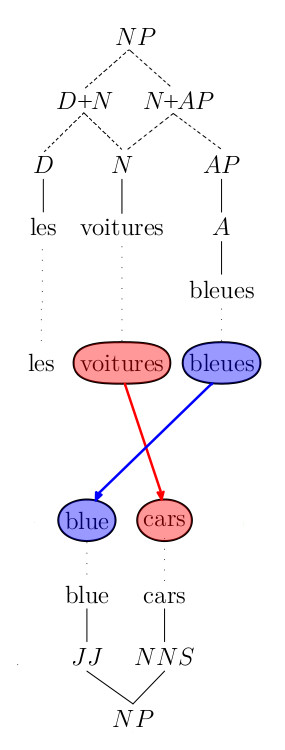
\includegraphics{rule-extr-2}}
\end{center}
\caption{\label{Fig-x} A fragment of Figure \ref{Fig-AlignedTreePair} with virtual nodes (symbolized by dashed lines) added on the French side.  Nodes D, N, and AP are all original children of the French NP.}
\end{figure}

We work through a small example of grammar extraction using Figure \ref{Fig-x}, which replicates a fragment of Figure \ref{Fig-AlignedTreePair} with virtual nodes included.  The English node JJ is aligned to the French nodes A and AP, the English node NNS is aligned to the French node N and the virtual node D+N, and the English node NP is aligned to the French node NP and the virtual node N+AP. To extract rules from the French node NP, we consider two potential decompositions: $D_1 = \{\text{D+N}, \text{AP}\}$ and $D_2 = \{\text{D}, \text{N+AP}\}$. Since the French NP is aligned only to the English NP, the set of left-hand sides is \{[NP]::[NP]\}, where we use the symbol ``::'' to separate the source and target sides of joint nonterminal label or a rule. 

In the next step, we use cached rules and alignments to generate all potential right-hand-side pieces from these top-level nodes:
$$
rhs(\text{D+N}) = \left\{
    \begin{array}{l}
    \lbrack\text{les voitures}]::[\text{cars}], \\
    \lbrack\text{D+N}^1]::[\text{NNS}^1] \\
    \end{array} \right\}
$$
$$
rhs(\text{AP}) =  \left\{ 
    \begin{array}{l}
    \lbrack\text{bleues}]::[\text{blue}], \\
    \lbrack\text{A}^1]::[\text{JJ}^1], \\
    \lbrack\text{AP}^1]::[\text{JJ}^1] \\
    \end{array} \right\}
$$
$$
rhs(\text{D}) = \emptyset
$$
$$
rhs(\text{N+AP}) = \left\{
    \begin{array}{l}
    \lbrack\text{N+AP}^1]::[\text{NP}^1], \\
    \lbrack\text{N}^1\ \text{JJ}^2]::[\text{AP}^2\ \text{NNS}^1], \\
    \lbrack\text{N}^1\ \text{JJ}^2]::[\text{A}^2\ \text{NNS}^1], \\
    \lbrack\text{voitures}\ \text{JJ}^1]::[\text{A}^1\ \text{cars}], \\
    \lbrack\text{voitures}\ \text{JJ}^1]::[\text{AP}^1\ \text{cars}], \\
    \lbrack\text{N}^1\ \text{bleues}]::[\text{blue}\ \text{NNS}^1], \\
    \lbrack\text{voitures bleues}]::[\text{blue cars}] \\
    \end{array} \right\}
$$
Next we must combine these pieces. For example, from $D_1$ we derive the full right-hand sides
\begin{enumerate}
\item {\em combine}([les voitures]::[cars], [bleues]::[blue]) \\= [les voitures bleues]::[blue cars]
\item {\em combine}([les voitures]::[cars], [A$^1$]::[JJ$^1$]) \\= [les voitures A$^1$]::[JJ$^1$ cars]
\item {\em combine}([les voitures]::[cars], [AP$^1$]::[JJ$^1$]) \\= [les voitures AP$^1$]::[JJ$^1$ cars]
\item {\em combine}([D+N$^1$]::[NNS$^1$], [bleues]::[blue])\\ = [ D+N$^1$ bleues]::[blue NNS$^1$]
\item{\em combine}([D+N$^1$]::[NNS$^1$], [A$^1$]::[JJ$^1$])\\ = [D+N$^1$ A$^2$]::[JJ$^2$ NNS$^1$]
\item {\em combine}([D+N$^1$]::[NNS$^1$], [AP$^1$]::[JJ$^1$] \\= [D+N$^1$ AP$^2$]::[JJ$^2$ NNS$^1$]
\end{enumerate}
Similarly, we derive eight full right hand sides from $D_2$.  Since $rhs(\text{D})$ is empty, rules derived have right-hand sides equivalent to $rhs(\text{N+AP})$ with the unaligned {\em les} added on the source side to complete the span of the French NP. For example, {\em combine}([N+AP$^1$]::[NP$^1$]) = [les N+AP$^1$]::[NP$^1$].

In the final step, the left-hand side is added to each full right hand side. Thus,
$$
\text{NP}::\text{NP} \rightarrow [\text{les voitures}\ \text{AP}^1]::[\text{JJ}^1\ \text{cars}]
$$
is one example rule extracted from this tree.

The number of rules can grow rapidly: if the parse tree has a branching factor of $b$ and a depth of $h$, there are potentially $O(2^{b^h})$ rules extracted [check?].  To control this, we allow certain constraints on the rules extracted that can short-circuit right-hand-side formation. We allow separate restrictions on the number of items that may appear on the right-hand side of phrase pair rules ($max_p$) and hierarchical grammar rules ($max_g$).  This is similar in spirit to the restriction in \newcite{GalleyEtAl-TTS} on the depth of extracted rules, but our constraints achieve the goal of controlling the rule length while remaining flexibile in terms of depth depending on the shape of the parse trees.  We also optionally allow for the exclusion of parallel unary rules --- that is, rules where the right-hand side consists solely of a pair of aligned non-terminals.


\section{Comparison to Other Methods}

\begin{table*}[tbh!]
\begin{center}
\begin{tabular}{l|llll}
 & {\bf Tree} & {\bf Multiple} & {\bf Virtual} & {\bf Multiple} \\
{\bf System} & {\bf Constraints} & {\bf Alignments} & {\bf Nodes} & {\bf Derivations} \\
\hline \hline
Hiero & No & --- & --- & Yes \\
Stat-XFER & ``Yes'' & No & Some & No* \\
GHKM & Yes & No & No & Yes \\
SAMT  & No & No? & Yes & ? \\
\newcite{Chiang-SourceAndTarget} & No & No & Yes & Yes \\
\hline
This work & Yes & Yes & Yes & Yes \\
\end{tabular}
\end{center}
\caption{\label{Table-Comparison} Comparisons between the rule extractor described in this paper and other existing SCFG rule extraction methods.}
\end{table*}

Table \ref{Table-Comparison} compares the rule extractor described in Section [x] to other SCFG extraction methods described in the literature.  We include comparisons of our work against the Hiero system \cite{Chiang-Hiero}, the Stat-XFER system rule learner most recently described by \newcite{AmbatiEtAl-ts2ts}, the composed version of GHKM rule extraction \cite{GalleyEtAl-TTS}, the so-called Syntax-Augmented MT (SAMT) system \cite{ZollmannVenugopal-SyntaxAugmentedMT}, and a Hiero--SAMT extension to source- and target-side syntax described by \newcite{Chiang-SourceAndTarget}.  Note that some of these methods make use of only target-side parse trees --- or no parse trees at all, in the case of Hiero --- but our primary interest in comparison is the constraints placed on the rule extraction process rather than the final output form of the rules themselves.  We highlight four specific dimensions along these lines.

{\bf Tree Constraints.}  As we mentioned in this paper's introduction, we do not allow any part of our extracted rules to violate constituent boundaries in the input parse trees.  This is in contrast to Hiero-derived techniques, which focus on expanding grammar coverage by extracting rules for all spans in the input sentence pair that are consistently word-aligned, regardless of their correspondence to linguistic constituents.  Practitioners of both phrase-based and syntax-based SMT have noticed severe grammar coverage issues when rules are required to exactly match parse constituents \cite{KoehnEtAl-PBSMT,Chiang-SourceAndTarget}.   In our work, we attempt to improve the coverage of the grammar by allowing multiple node alignments, virtual nodes, and multiple tree decompositions rather than ignoring structure constraints.

{\bf Multiple Alignments.}  In contrast to all other extraction methods in Table \ref{Table-Comparison}, ours allows a node in one parse tree to be aligned with multiple nodes in the other tree, as long as the word-alignment and structure constraints are satisfied.  However, we do not allow a node to have multiple simultaneous alignments --- a single node alignment must be chosen for extracting an individual rule.  In practice, this prevents extraction of ``triangle'' rules where the same node appears on both the left- and right-hand side of the same rule.

{\bf Virtual Nodes.}  In keeping with our philosophy of representing multiple alignments, our use of multiple and overlapping virtual nodes is less restrictive than the single-alignment constraint of Stat-XFER.  Another key difference is that Stat-XFER requires all virtual nodes to be aligned to original nodes in the other language, while we permit virtual--virtual node alignments.  Again, in respecting existing tree structure constraints, our virtual node placement is more restrictive than SAMT or Chiang, where extracted nodes may cross existing constituent boundaries.

{\bf Multiple Derivations.}  \newcite{GalleyEtAl-TTS} argued that breaking a single tree pair into multiple decompositions [is important for ------].  We agree, and we base our rule extractor's acquisition of multiple derivations per tree pair on techniques from both GHKM and Hiero extraction.  More specifically, we borrow from Hiero the idea of creating hierarchical rules by subtracting and abstracting smaller phrases (aligned nodes in our case) from larger phrases.  Like GHKM, we do this exhaustively within some limit, although in our case we use a rank limit on a rule's right-hand side rather than a limit on the depth of the subnode subtractions.


\section{Experiments}

We conducted experiments with our rule extractor on the FBIS corpus, made up of approximately 302,000 Chinese--English sentence pairs.  We parsed the corpus with the Chinese and English grammars of the Berkeley parser \cite{Berkeley-Parser} and word-aligned it with [ask Chris Dyer].  The parsed and word-aligned corpus served as the input to our rule extractor, which we ran with a number of different settings.  First, we acquired a baseline rule extraction from our corpus using an implementation of the basic Stat-XFER rule learner \cite{Lavie-SSST}, which decomposes each input tree pair into a single set of minimal SCFG rules using only original nodes in the parse trees.  Next, we tested the effect of allowing multiple decompositions by running our own rule learner, but restricting its rules to also only make use of original nodes.  Finally, we investigated the total number of extractable rules by allowing the creation of virtual nodes from up to four adjacent sibling nodes and placing two different limits on the length of the right-hand side.  These configurations are summarized in Table \ref{Table-RuleSets}.

\begin{table}[tbh!]
  \begin{tabular}{lrrll}
  {\bf Rule Set} & {\bf $max_p$} & {\bf $max_g$} & {\bf Virtual} & {\bf Unary} \\
  \hline \hline
  xfer-orig  &  ? & $\infty$ & No & Yes \\
  compatible & 10 & 5 & No & Yes \\
  \hline
  full-short &  5 & 5 & Yes & No \\
  full-long  &  7 & 7 & Yes & No \\
%%  short-instance & 5 & 5 & All & No & All instances \\
%%  short-uniq & 5 & 5 & All & No & Unique rules\\
%%  short-100k & 5 & 5 & All & No & 100000 top grammar rules\\
%%  short-10k & 5 & 5 & All & No & 10000 top grammar rules\\
%%	long-instance	& 7 & 7	& All & No & All instances \\
%%	long-uniq	& 7 & 7	& All & No & Unique rules \\
%%	long-100k & 7 & 7 & All & No & 100000 top grammar rules\\
%%  long-10k & 7 & 7 & All & No & 10000 top grammar rules\\
  \end{tabular}
  \caption{\label{Table-RuleSets} Rule sets considered}
\end{table}

\subsection{Rules Extracted}

\begin{table*}[tbh!]
\begin{center}
\begin{tabular}{l|rr|rr}
 & \multicolumn{2}{c|}{{\bf Extracted Instances}} & \multicolumn{2}{c}{{\bf Unique Rules}} \\
{\bf Rule Set} & {\bf Phrase} & {\bf Hierarchical} & {\bf Phrase} & {\bf Hierarchical} \\
\hline \hline
xfer-orig  &  6,152,389 &  1,876,384  &  1,450,262 &    767,573 \\
compatible & &  &  & \\
\hline
full-short & 10,190,487 & 14,190,066  &  2,877,650 &  8,313,690 \\
full-long  & 10,288,731 & 22,479,863  &  2,970,403 & 15,750,695 \\
\end{tabular}
\end{center}
\caption{\label{Table-NumRules} x}
\end{table*}

As expected, we find that allowing multiple decompositions of each tree pair has a significant effect on the number of extracted rules.  Table \ref{Table-NumRules} shows [something when it's all filled in]

[Here can we include the venn diagram info?]

======

The breakdown by size of node is shown in Table

\begin{table}
\begin{tabular}{c|rrrrrrr|r}
&1&2&3&4&5&Total\\
\hline
1&0&124836&78161&34657&14931&6673&3197&262455\\
2&47362&803748&386908&150704&60073&24259&9853&1482907\\
3&17716&236120&1253785&457095&154331&58123&23644&2200814\\
4&5359&53885&331222&1478123&467530&155063&59036&2550218\\
5&1742&13542&68144&422119&1651904&511449&152677&2821577\\
6&697&4544&17223&91029&527639&1937370&496569&3075071\\
7&276&1614&5450&23108&119798&678834&2528573&3357653\\
\hline
Total&73152&1238289&2140893&2656835&2996206&3371771&3273549&15750695\\
\end{tabular}
\caption{Rule length distribution for rule set long-uniq}
\end{table}

\begin{table}
\begin{tabular}{r|rrrrr|r}
&1&2&3&4&5&Total\\
\hline
1&0&471&14&1&0&486\\
2&114&5394&694&77&6&6285\\
3&3&206&2084&112&6&2411\\
4&0&3&61&568&11&643\\
5&0&0&0&48&153&201\\
\hline
Total&117&6074&2853&806&176&1002\\
\end{tabular}
\caption{Rule length distribution for rule set short-10k}
\end{table}

\begin{table}[tbh!]
  \begin{tabular}{lrrr}
  Rule Set & \# LHS Type OO & Total Phrase Rules & \% Type OO\\
  \hline
  short-uniq & 1955803 & 2877650 & 67.96528417\\
	short-instance & 8646129 & 10190487 & 84.84510112\\
	long-uniq	& 2015093 & 2970403	& 67.83904406\\
	long-instance & 8709046	& 10288731 & 84.64645446\\
  \end{tabular}
  \caption{Original rules for phrase nodes}
\end{table}

\begin{table}[tbh!]
  \begin{tabular}{lrrr}
  Rule Set & \# LHS Type OO & Total Grammar Rules & \% Type OO\\
  \hline
  short-uniq	& 3791489 &	8313690	& 45.60536898\\
  short-instance &	6494567 &	14190066 & 45.76840587\\
  long-uniq &	7086016 &	15750695 & 44.98859257\\
  long-instance & 10124262 & 22479863 & 45.03702714\\
  short-10k & 4650 & 10026 & 46.37941352\\
  short-100k & 50618 & 106402 & 47.57241405\\
  long-10k & 4583 & 10023 & 45.72483288\\
  long-100k & 47457 & 109082 & 43.50580297
  \end{tabular}
  \caption{Original rules for grammar nodes}
\end{table}

\subsection{Translation results}

We used these rule sets to obtain the following 
translation results.

\begin{table}[tbh!]
\begin{tabular}{llrrr}
Rule Set & Test Set & BLEU & TER & Meteor \\
\hline
short-10k & mt03 & 25.16 & 66.25 & 54.33 \\
short-100k & mt03 & 25.51 & 65.56 & 54.15 \\
long-10k & mt03 & 25.74  & 65.52 & 54.55 \\
long-100k & mt03 & 25.53 & 66.24 & 53.68 \\
\hline
short-10k & mt08 & 19.30  & 66.57 & 46.26\\
short-100k & mt08 & 19.22 & 66.16 & 45.62\\
long-10k & mt08 & 19.04  & 66.20 & 46.25\\
long-100k & mt08 & 19.12 & 67.02 & 45.26\\
\end{tabular}
\caption{Translation evaluation results on the extracted rule sets.}
\end{table}

\bibliography{syntax-mt}


\end{document}
